\label{chap:financeiro}
A análise de de demonstrações financeiras é composta pelas análises de \emph{fluxo de caixa}, do \emph{demonstrativo de resultados} e a da \emph{por meio de índices}, as quais embasam a demonstração financeira da companhia em questão.

\section{Fluxo de caixa}

A respeito do seguinte do fluxo de caixa, que consta completo no apêndice \ref{sec:fluxoDeCaixa}

\begin{enumerate}
\item  A empresa gerou caixa bruto positivo ou negativo? Por quê? Graças ao Lucro ou aos ajustes (depreciação)?\\ Nos 3 anos, ou seja, em 2015, 2016 e 2017 ela gerou caixa bruto positivo. No ano de 2015, a Positivo só gerou caixa bruto positivo, devido aos ajustes / depreciação, porém como a Positivo, trabalha com matéria prima importada, ela sofre muito com a variação cambial, e em 2015, a variação cambial foi muito grande, e ela se protegeu bem, se não o resultado poderia ser pior. No ano subsequente, apesar de ter havido grandes perdas com variação cambial, a Positivo gerou caixa bruto positivo com sua eficiência operacional. E, finalmente, em 2017 a Positivo não apresentou uma boa eficiência operacional e teve grandes perdas com variação cambial, portanto, só gerou caixa bruto positivo graças a depreciação e/ou amortização.

\item A empresa gerou ou consumiu caixa com o giro? Por quê? \\ Em 2015 a Positivo gerou caixa positivo com capital de giro, com contas a receber e estoques. Já em 2016 a geração de caixa com capital de giro foi negativa devido ao aumento do estoque. \\ Como em 2016, em 2017 a geração de caixa com capital de giro foi negativa devido ao aumento do estoque.

\item A empresa gerou ou consumiu caixa com os investimentos? Por quê? \\ Nos três anos de exercício, a Positivo consumiu caixa com os investimentos, mesmo tendo o valor positivo de recebimento de dividendos em 2015, os valores para aquisição de imobilizado e o Aumento de Intangível foram inversamente negativos e tiveram um peso maior na influência do consumo do caixa operacional da empresa.

\item A empresa gerou ou consumiu caixa com os financiamentos? Por quê? \\ A Positivo só gerou caixa com financiamentos em 2015, já em 2016 e 2017 a empresa adotou a estratégia de diminuir o endividamento e com isso, consumiu caixa com financiamento.

\item Qual sua decisão sobre esta empresa? \\ Em função da crise instalada no Brasil desde 2013, a Positivo não teve um bom resultado no ano de 2015, porém aproveitou para investir. No ano seguinte, 2016, a Positivo teve um ano excepcional, recuperando o que foi investindo no ano anterior e adotando uma estratégia de diminuição de dívidas. Por fim, em 2017, o ano não foi tão bom, porém a empresa continuou na sua estratégia de diminuição de dívidas.
\end{enumerate}

\section{Análise Vertical: Balanço Patrimonial}

Na Análise Vertical do Balanço Patrimonial os pontos a serem analisados são do valor de Caixa, de Estoques e de Contas a Receber por possuírem a proporção maior no impacto dos resultados do balanço. 

\begin{table}[h]
\begin{centering}
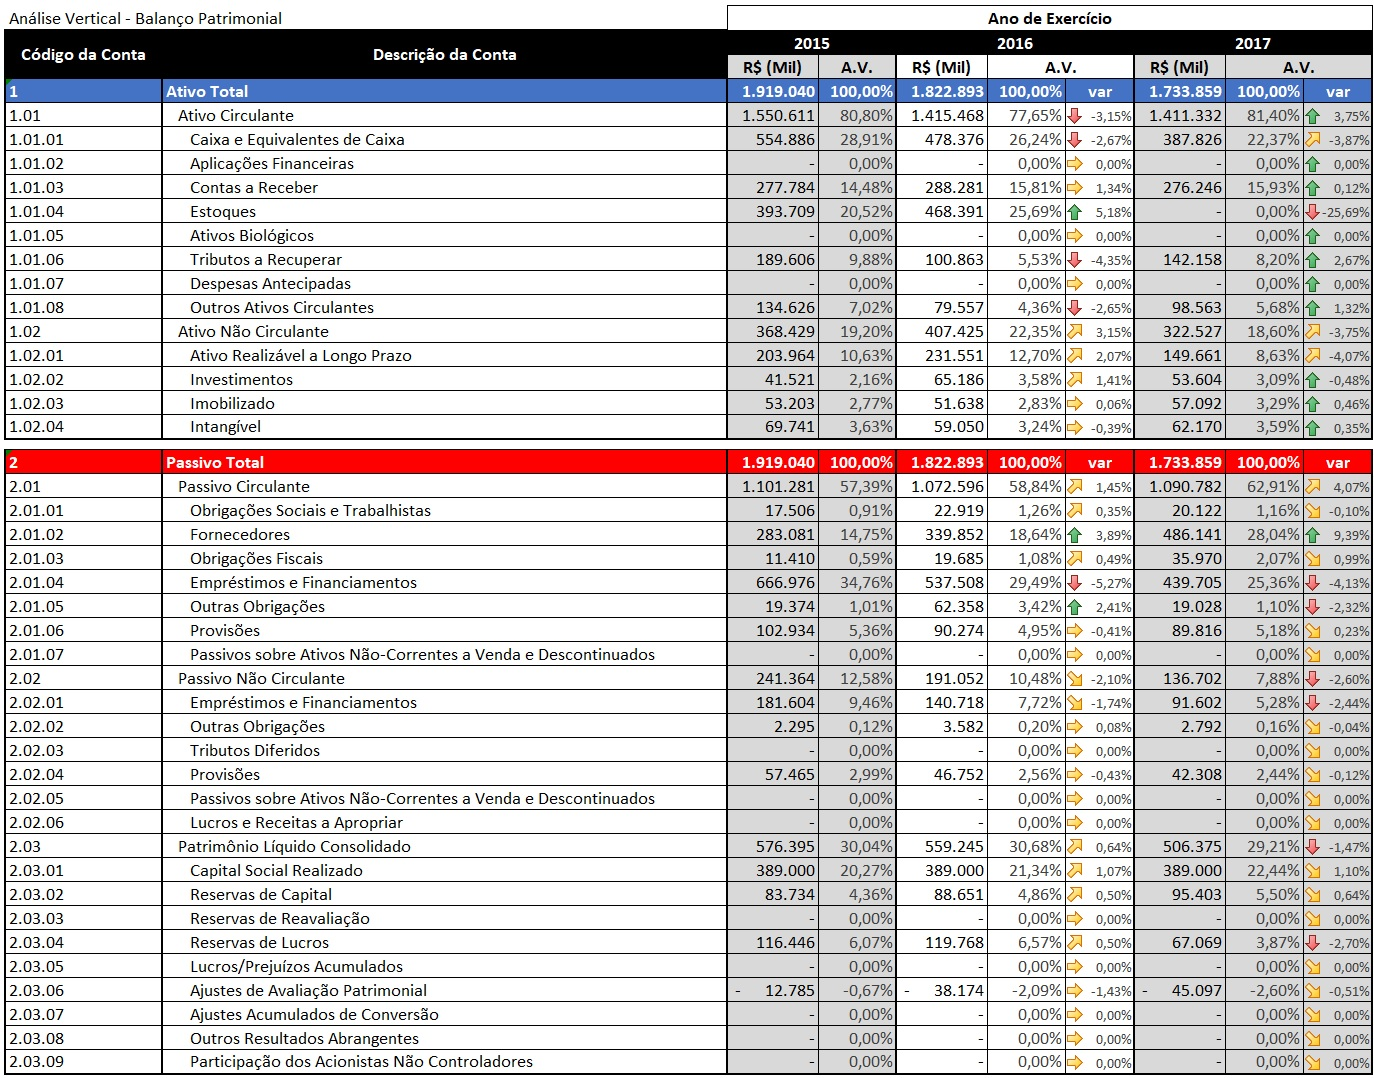
\includegraphics[width=1.0\textwidth]{Img/AnaliseVerticalBalancoPatrimonial}
\caption{Análise Vertical do Balanço Ativo para os anos de 2015, 2016 e 2017.}
\par\end{centering}
\end{table}

%\begin{center}
%\begin{table}[h]
  %%\begin{tabular}{>{\raggedright}p{0.15\textwidth}|>{\raggedright}p{0.3\textwidth}|>{\raggedright}p{0.08\textwidth}>{\raggedright}p{0.08\textwidth}>{\raggedright}p{0.08\textwidth}}
%\begin{tabular}{p{.15\textwidth}|p{.35\textwidth}|p{.10\textwidth}|p{.10\textwidth}|p{.10\textwidth}}
%\hline 
 %& (Reais Mil) & \multicolumn{3}{c}{Ano de Exercício}\tabularnewline
%\hline 
%Id Conta & Descrição da Conta & 2017 & 2016 & 2015\tabularnewline
%\hline 
%1 & Ativo Total & 1.733.859 & 1.822.893 & 1.919.040\tabularnewline
%1.01.01 & Caixa e Equivalentes de Caixa & 387.826 & 478.376 & 554.886\tabularnewline
%1.01.02 & Aplicações Financeiras & 0 & 0 & 0\tabularnewline
%1.01.03 & Contas a Receber & 276.246 & 288.281 & 277.784\tabularnewline
%1.01.04 & Estoques & 506.539 & 468.391 & 393.709\tabularnewline
%1.01.05 & Ativos Biológicos & 0 & 0 & 0\tabularnewline
%1.01.06 & Tributos a Recuperar & 142.158 & 100.863 & 189.606\tabularnewline
%1.01.07 & Despesas Antecipadas & 0 & 0 & 0\tabularnewline
%1.01.08 & Outros Ativos Circulantes & 98.563 & 79.557 & 134.626\tabularnewline
%1.02.01 & Ativo Realizável a Longo Prazo & 149.661 & 231.551 & 203.964\tabularnewline
%1.02.02 & Investimentos & 53.604 & 65.186 & 41.521\tabularnewline
%1.02.03 & Imobilizado & 57.092 & 51.638 & 53.203\tabularnewline
%1.02.04 & Intangível & 62.170 & 59.050 & 69.741\tabularnewline
%\hline 
%\end{tabular}
%\caption{\label{tab:balancoAtivo} Análise Vertical do \emph{Balanço Ativo} para  os anos de 2015, 2016 e 2017.}
%\end{table}
%\vspace*{-40pt}
%\par\end{center}

%\begin{center}
%\begin{table}[h]
%\begin{tabular}{p{.15\textwidth}|p{.35\textwidth}|p{.10\textwidth}|p{.10\textwidth}|p{.10\textwidth}}
%\hline 
 %& (Reais Mil) & \multicolumn{3}{c}{Ano de Exercício}\tabularnewline
%\hline 
%Id Conta & Descrição da Conta & 2017 & 2016 & 2015\tabularnewline
%\hline 
%\textbf{1} & \textbf{Ativo Total} & \textbf{100.00\%} & \textbf{100.00\%} & \textbf{100.00\%}\tabularnewline
%1.01.01 & Caixa e Equivalentes de Caixa & 22.37\% & 26.24\% & 28.91\%\tabularnewline
%1.01.02 & Aplicações Financeiras & 0.00\% & 0.00\% & 0.00\%\tabularnewline
%1.01.03 & Contas a Receber & 15.93\% & 15.81\% & 14.48\%\tabularnewline
%1.01.04 & Estoques & 29.21\% & 25.69\% & 20.52\%\tabularnewline
%1.01.05 & Ativos Biológicos & 0.00\% & 0.00\% & 0.00\%\tabularnewline
%1.01.06 & Tributos a Recuperar & 8.20\% & 5.53\% & 9.88\%\tabularnewline
%1.01.07 & Despesas Antecipadas & 0.00\% & 0.00\% & 0.00\%\tabularnewline
%1.01.08 & Outros Ativos Circulantes & 5.68\% & 4.36\% & 7.02\%\tabularnewline
%1.02.01 & Ativo Realizável a Longo Prazo & 8.63\% & 12.70\% & 10.63\%\tabularnewline
%1.02.02 & Investimentos & 3.09\% & 3.58\% & 2.16\%\tabularnewline
%1.02.03 & Imobilizado & 3.29\% & 2.83\% & 2.77\%\tabularnewline
%1.02.04 & Intangível & 3.59\% & 3.24\% & 3.63\%\tabularnewline
%\hline
%\end{tabular}
%\caption{\label{tab:balancoAtivo} Análise Vertical das contribuições percentuais em relação ao \emph{Balanço Ativo} (tabela \ref{tab:balancoAtivo}) para  os anos de 2015, 2016 e 2017.}
%\end{table}
%\vspace*{-40pt}
%\par\end{center}

\subsection{Caixa}
O ponto positivo no caso do valor de Caixa é que pode-se dizer que a Positivo gerou caixa nos três últimos exercícios analisados e aparenta estar com sua gestão de fluxo saudável, porém, há uma diminuição de 6,54 p.p. em comparação ao exercício de 2015, o que pode levar a crer que por motivos economicos do país ou internos a empresa não está conseguindo manter a força na geração deste caixa.

\subsection{Estoque}
Já no caso do valores de estoque há um significativo aumento de 8,69 p.p. no exercício de 2017 com relação ao exercício de 2015. Neste caso, pode-se analisar de duas maneiras: a primeira é que a Positivo quer aproveitar a onda de alta que o mercado de vendas de PC apresenta desde o 2º trimestre de 2017 e por isso aumentou seu valor de estoque para poder aumentar seu poder de venda; a segunda é que analisando o Ativo Total da empresa percebe-se um declínio no exercício de 2017 em comparação aos demais exercícios. Na junção de análises de diminuição de Caixa e de Ativo Total da empresa, faz mais sentido prever que esse aumento de Estoque está relacionado a má fluidez de vendas no período.

\subsection{Contas a Receber}

O aumento de 1,45 p.p. do exercício de 2017 em relação ao exercício de 2015 mostra que a empresa vem captando mais recursos dos clientes por meio de pagamentos à prestações. Parte desse aumento das Contas a Receber explica a diminuição da geração do caixa a cada exercício, mas não em sua totalidade visto que a diferença dos anos anteriores não é muito expressiva. Deste modo, pode-se considerar que a empresa está utilizando de outros meios de captação de recursos para não perder volume de vendas e talvez, numa análise que precisa de mais embasamento, justificar o leve aumento de 0,52 p.p de imobilizados no exercício de 2017 em relação ao de 2015.

\section{Demonstrativo de Resultados do Exercício}

\begin{table}[h]
\begin{centering}
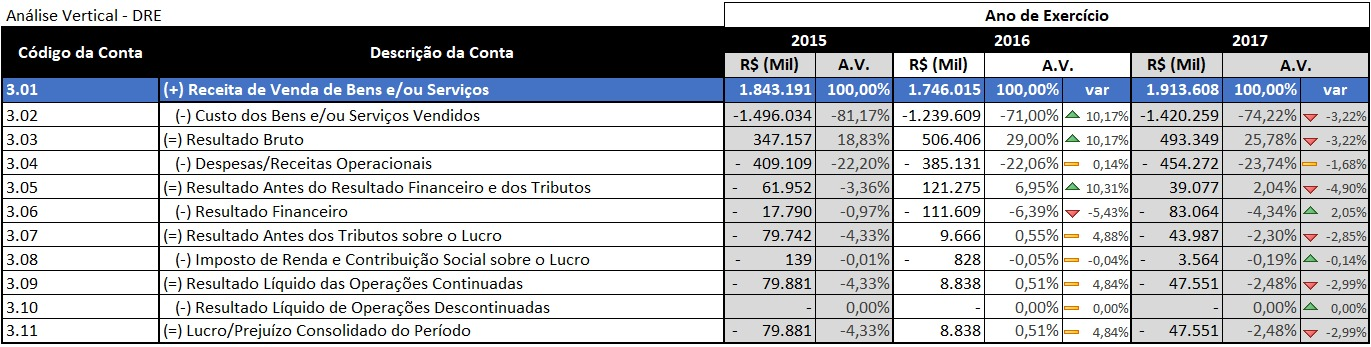
\includegraphics[width=1.0\textwidth]{Img/AnaliseVerticalDre}
\caption{Tabela de análise do DRE com relação aos anos exercícios de 2015, 2016 e 2017.}
\par\end{centering}
\end{table}

Na análise das Demonstrações de Resultados dos três exercícios propostos, a Positivo apresentou melhora considerável na receita da venda de bens e diminuiu seus custos a fim de obter um resultado bruto mais ajustável ao longo do período. 

As despesas operacionais da empresa aumentaram e acarretaram na diminuição de 4,91 p.p. no Resultado Antes do Resultado Financeiro e dos Tributos em relação ao exercício de 2016. Mesmo com a melhora do Resultado Financeiro no exercício de 2017, a empresa ainda continuou com esse indicador no negativo o que acabou contribuindo para o prejuízo mesmo antes do abatimento do imposto de renda e contribuições sociais do período.

Tende-se a considerar que o país passou por dificuldades econômicas e contribuiu nas oscilações dos resultados da empresa que já apresentavam melhora no exercício de 2016 em relação ao do ano anterior.

A empresa fechou com prejuízo no período, mas indica melhora nos resultados pelo fato da diminuição das despesas operacionais e financeiras, aumento da receita de venda, aumento do resultado bruto e um ponto principal que foi a diminuição das despesas com flutuações cambiais que é um ponto fraco da instituição.

\section{Análise por Meio de Índices}
\label{sec:analiseIndices}

Para a análise por meio de índices será utilizado os indicadores de \emph{liquidez}.

\subsection{Indicadores de Liquidez}

\begin{table}[h]
\begin{centering}
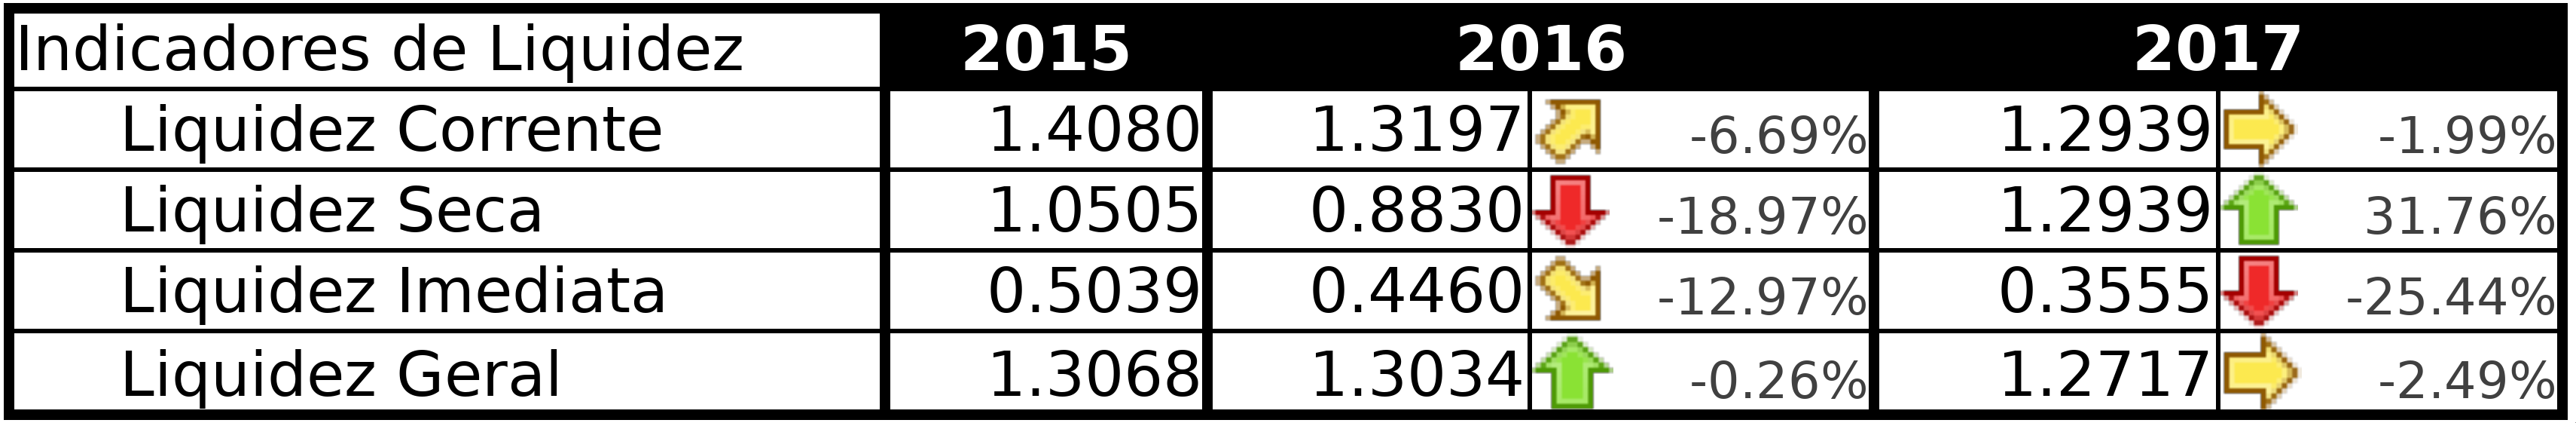
\includegraphics[width=1.0\textwidth]{Img/IndicadorLiquidez}
\caption{\label{tab:indicadorLiquidez}Tabela dos indicadores de liquidez para os anos de 2015, 2016 e 2017.}
\par\end{centering}
\end{table}

Quando o valor é maior que 1, demonstra-se que há capital disponível para uma possível liquidação das obrigações. Se for igual a 1, os direitos e obrigações a curto prazo são equivalentes. No caso de ser menor que 1, a empresa não teria capital disponível suficiente para quitar as obrigações a curto prazo, caso fosse preciso.

Quanto aos indicadores de liquidez, são as equações:

\begin{equation}
  Liquidez_{Corrente}=\frac{Ativo_{Circulante}}{Passivo_{Circulante}}
  \label{eq:liquidezcorrente}
\end{equation}

\begin{equation}
  Liquidez_{Seca} = \frac{Ativo_{Circulante} – Estoques}{Passivo_{Circulante}}
  \label{eq:liquidezseca}
\end{equation}

\begin{equation}
  Liquidez_{Imediata} = \frac{{Disponível}}{Passivo_{Circulante}}
  \label{eq:liquidezseca}
\end{equation}

\begin{equation}
  Liquidez_{Geral} = \frac{(Ativo_{Circulante} + Realizável_{Longo Prazo})}{(Passivo_{Circulante} + Exigível_{Longo Prazo})}
  \label{eq:liquidezgeral}
\end{equation}

Utilizou-se os indicadores de liquidez para avaliar a capacidade de pagamento do empréstimo pela empresa solicitante, de tal forma a compararmos as suas obrigações junto a fornecedores e funcionários. Para uma ampla e abrangente análise de liquidez da empresa, optou-se por estudar os quatro índices de forma simultânea e comparativa, a partir dos resultados de ativo e passivo, obtidos no balanço patrimonial, disponíveis no apêndice \ref{sec:balancoAtivo} e \ref{sec:balancoPatrimonial}.

Tais indicadores, observados na tabela \ref{tab:indicadorLiquidez} direcionaram no sentido de concessão do empréstimo, já que após a análise desses indicadores, classificamos como \emph{baixo} o risco em relação ao futuro da empresa. Os demonstrativos indicam que a solicitante possui capital e/ou previsão disponível para a liquidação das obrigações futuras.
